\documentclass[11pt,a4paper, 
swedish, english %% Make sure to put the main language last!
]{article}
\pdfoutput=1

%% Andréas's custom package 
%% (Will work for most purposes, but is mainly focused on physics.)
\usepackage{../custom_as}
\usepackage{mathrsfs}
\usepackage{eufrak}
\usepackage{cancel}
%% Figures can now be put in a folder: 
\graphicspath{ {figures/} %{some_folder_name/}
}
\usepackage{multicol}

%% If you want to change the margins for just the captions
\usepackage[size=small]{caption}

%% To add todo-notes in the pdf
\usepackage[%disable  %%this will hide all notes
]{todonotes} 

%% Change the margin in the documents
\usepackage[
%            top    = 3cm,              %% top margin
%            bottom = 3cm,              %% bottom margin
%            left   = 3cm, right  = 3cm %% left and right margins
]{geometry}

\newcommand{\enull}{\ensuremath{\varepsilon_{0}}}
\newcommand{\lD}{\ensuremath{\lambda_{\text{D}}}}
\newcommand{\wc}{\ensuremath{\omega_{\text{c}}}}
\newcommand{\rhom}{\ensuremath{{\rho_{\text{m}}}}}
\newcommand{\vA}{\ensuremath{v_{\text{A}}}}
\newcommand{\cs}{\ensuremath{c_{\text{s}}}}


%% If you want to chage the formatting of the section headers
\renewcommand{\thesubsection}{\arabic{section}.\Alph{subsection}}



%%%%%%%%%%%%%%%%%%%%%%%%%%%%%%%%%%%%%%%%%%%%%%%%%%%%%%%%%%%%%%%%%%%%%%
\begin{document}%% v v v v v v v v v v v v v v v v v v v v v v v v v v
%%%%%%%%%%%%%%%%%%%%%%%%%%%%%%%%%%%%%%%%%%%%%%%%%%%%%%%%%%%%%%%%%%%%%%


%%%%%%%%%%%%%%%%%%%% vvv Internal title page vvv %%%%%%%%%%%%%%%%%%%%%
\title{Assignment 4 \\
{\Large Plasma Physics -- RRY085}}
\author{Andréas Sundström}
\date{2017-10-15}

\maketitle

%%%%%%%%%%%%%%%%%%%% ^^^ Internal title page ^^^ %%%%%%%%%%%%%%%%%%%%%
%% If you want a list of all todos
%\todolist

\section{Collisional diffusion in weakly ionized gas}
Assume that the electron-neutral interaction rate is
\begin{equation}
\nu_{\text{en}}=v_\ee N \sigma_\text{en},
\end{equation}
and the electron-ion interaction rate is
\begin{equation}
\nu_\text{ei}=\frac{\pi n e^4}{(4\pi\varepsilon_0 m_\ee)^2v_\ee^3},
\end{equation}
where $N$ is the neutral particle density and $n=n_\ee=n_\text{i}$ is
the electron/ion density. Then
\begin{equation}
\frac{\nu_\text{ei}}{\nu_{\text{en}}}
=\frac{n}{N}\frac{e^4}
{16\pi\varepsilon_0^2\sigma_\text{en}m_\ee^2 v_\ee^4}.
\end{equation}
If we take $\sigma_\text{en}=\unit[10^{-19}]{m^2}$ and an electron
energy of 1\,eV, then for the two different frequencies to be equal,
we would require 
\begin{equation}
\frac{n}{N}=
\frac{64\pi\varepsilon_0^2
\sigma_\text{en}\,\epsilon^2}{e^4}
\approx 0.06 = 6\,\%,
\end{equation}
where $\epsilon =m_\ee v_\ee^2/2$ is the energy of an electron.

Given air normal atmospheric pressure at room temperature with
$N=\unit[10^{26}]{m^{-3}}$ and weakly ionized plasma, and with the
same electron energy and $\sigma_\text{en}$. Then the diffusion
constant is roughly 
\begin{equation}
D=\frac{v_\ee^2}{\nu_\text{en}}
=\frac{v_\ee}{N\sigma_\text{en}}
=\frac{1}{N\sigma_\text{en}}\sqrt{\frac{2\epsilon}{m_\ee}}
\approx \unit[0.06]{m^2/s}.
\end{equation}
Since the plasma would be weakly ionized the electron-neutral
collision rate dominates. 



\section{Different heat conductivity models}
In this problem we're considering a 1D plasma system, and we will
investigate how different types of heat conductivity, $\chi$, will
affect the temperatures of the plasma. The temperature is given by the
ODE
\begin{equation}
\dv{r}\qty[\chi\dv{T}{r}]=-S(r)\qc
\eval{\dv{T}{r}}_{r=0}=0\qc
T(r=R)=T_0,
\end{equation}
where $S(r)=S_0(r-r_0)$ with $0<r_0<R$. With this information, we can
integrate both sides once
\begin{equation}\label{eq2:ODE}
\chi\dv{T}{r}=-S_0\Theta(r-r_0),
\end{equation}
where $\Theta$ is the Heaviside step function. There should also be a
constant of integration here, but with the initial condition
$\eval{\dv*{T}{r}}_{r=0}=0$, we see that said constant has to be~0
(unless $\chi$ diverges at $r\to0$).

Seeing that we will be dealing with the Heaviside step function, we
might as well state the following identity for finding primitive
functions to a product with the step function. Given some (smooth)
function $f(x')$ and the constants $x_1<x_0$, then 
\begin{equation}
\begin{aligned}
\int_{x_1}^{x}\dv{f}{x'}\Theta(x'-x_0)\id{x'}=&
\Theta(x-x_0)\int_{x_0}^{x}\dv{f}{x'}\id{x'}
=\Big(f(x)-f(x_0)\Big)\Theta(x-x_0).
\end{aligned}
\end{equation}
Obviously, any primitive function to $(\dv*{f}{x'})\Theta(x'-x_0)$
will be given by the RHS plus some arbitrary constant, thus
\begin{equation}\label{eq2:heaviside-int}
\int\dv{f}{x}\Theta(x-x_0)\id{x}
=C+\Big(f(x)-f(x_0)\Big)\Theta(x-x_0).
\end{equation}



\subsection{Classical transport}
If the heat conductivity follows classical heat transport, then
\begin{equation}
\chi(T)=\alpha_1T^{-1/2}
\end{equation}
and \eqref{eq2:ODE} is separable and we get
\begin{equation}
\int\alpha_1T^{-1/2}\id{T}=-\int S_0\Theta(r-r_0)\id{r},
\end{equation}
which, by \eqref{eq2:heaviside-int}, becomes
\begin{equation}
T^{1/2}(r)=\mathcal{T}^{1/2}
-\frac{S_0}{2\alpha_1}(r-r_0)\Theta(r-r_0).
\end{equation}
The constant of integration, $\mathcal{T}^{1/2}$, can easily be
determined by the boundary condition $T(r=R)=T_0$ which yields
\begin{equation}\label{eq2a:const}
T_0^{1/2}=\mathcal{T}^{1/2}-\frac{S_0}{2\alpha_1}(R-r_0)
\quad\Longleftrightarrow\quad
\mathcal{T}^{1/2}=T_0^{1/2}+\frac{S_0}{2\alpha_1}(R-r_0).
\end{equation}
This means that the temperature is
\begin{equation}
T(r)=\qty{T_0^{1/2}+\frac{S_0}{2\alpha_1}
\Big[(R-r_0)-(r-r_0)\Theta(r-r_0)\Big]}^2
\end{equation}
With words, the temperature stays constant $T=\mathcal{T}$, given by
\eqref{eq2a:const}, up until $r=r_0$ when the temperature drops 
``quadratically'' (along a parabola whose vertex is just to the right
of $r=R$) down to $T=T_0$ at $r=R$. 

\subsection{Neoclassical transport}
With neoclassical transportation, the heat conductivity is
\begin{equation}
\chi(r, T)=
\begin{cases}
\alpha_2 r_1^{-3/2}T^{-1/2}\qc&0\le r<r_1\\
\alpha_2 r^{-3/2}T^{-1/2}\qc& r_1\le r\le1,
\end{cases}
\end{equation}
where $0<r_1<r_0$. 

It is obvious that the temperature, just as before, will be constant
$T(r)=\mathscr{T}$ for $0\le r<r_0$ since $\dv*{T}{r}=0$ in that region. We
therefore only have to focus on the (overlapping) region
$r_1<r<R$. Here \eqref{eq2:ODE} 
%can be rewritten as 
%\begin{equation}
%\alpha_2T^{-1/2}\dv{T}{r}=-S_0\,r^{3/2}\Theta(r-r_0)=-S_0\,r^{3/2}
%\end{equation}
%which 
separates into
\begin{equation}
\alpha_2\int T^{-1/2}\id{T}=-S_0\int r^{3/2}\Theta(r-r_0) \id{r}.
\end{equation}
By \eqref{eq2:heaviside-int}, we therefore get
\begin{equation}
T^{1/2}(r)=\mathscr{T}^{1/2}
-\frac{S_0}{5\alpha_2}\qty(r^{5/2}-r_0^{5/2})\Theta(r-r_0).
\end{equation}
Once again, the constant $\mathscr{T}^{1/2}$ is determined by the boundary
condition $T(r=R)=T_0$, which yields
\begin{equation}
\mathscr{T}^{1/2}=T_0^{1/2}+
\frac{S_0}{5\alpha_2}\qty(R^{5/2}-r_0^{5/2}).
\end{equation}
Therefore
\begin{equation}
T(r)=\qty{T_0^{1/2}+\frac{S_0}{5\alpha_2}
\qty[\qty(R^{5/2}-r_0^{5/2})-\qty(r^{5/2}-r_0^{5/2})\Theta(r-r_0)]}^2.
\end{equation}
This is harder to describe with words, but the temperature is constant
$T=\mathscr{T}$ for $0\le r<r_0$ and then it starts dropping down to
$T(R)=T_0$. 

\subsection{Turbulent Gyro-Bohm like transport}
For turbulent Gyro-Bohm like transport, the heat conductivity is given
by
\begin{equation}
\chi(T)=\alpha_3 T^{3/2}.
\end{equation}
Thus, \eqref{eq2:ODE} separates into
\begin{equation}
\alpha_3\int T^{3/2}\id{T}=-S_0\int \Theta(r-r_0) \id{r}.
\end{equation}
As usual, \eqref{eq2:heaviside-int} gives
\begin{equation}
T^{5/2}(r)=\mathfrak{T}^{5/2}
-\frac{5S_0}{2\alpha_3}\qty(r-r_0)\Theta(r-r_0).
\end{equation}
The boundary condition $T(r=R)=T_0$ yields
\begin{equation}
\mathfrak{T}^{5/2}=T_0^{5/2}+
\frac{5S_0}{2\alpha_3}\qty(R-r_0)
\end{equation}
wherefore
\begin{equation}
T(r)=\qty{T_0^{5/2}+\frac{5S_0}{2\alpha_3}
\Big[(R-r_0)-(r-r_0)\Theta(r-r_0)\Big]}^{2/5}.
\end{equation}
Once again, this is constant $T=\mathfrak{T}$ for $0\le r<r_0$, and
then the temperature drops down to $T_0$ at $r=R$.

\subsection*{Limiting type of transport}
\begin{figure}
\centering
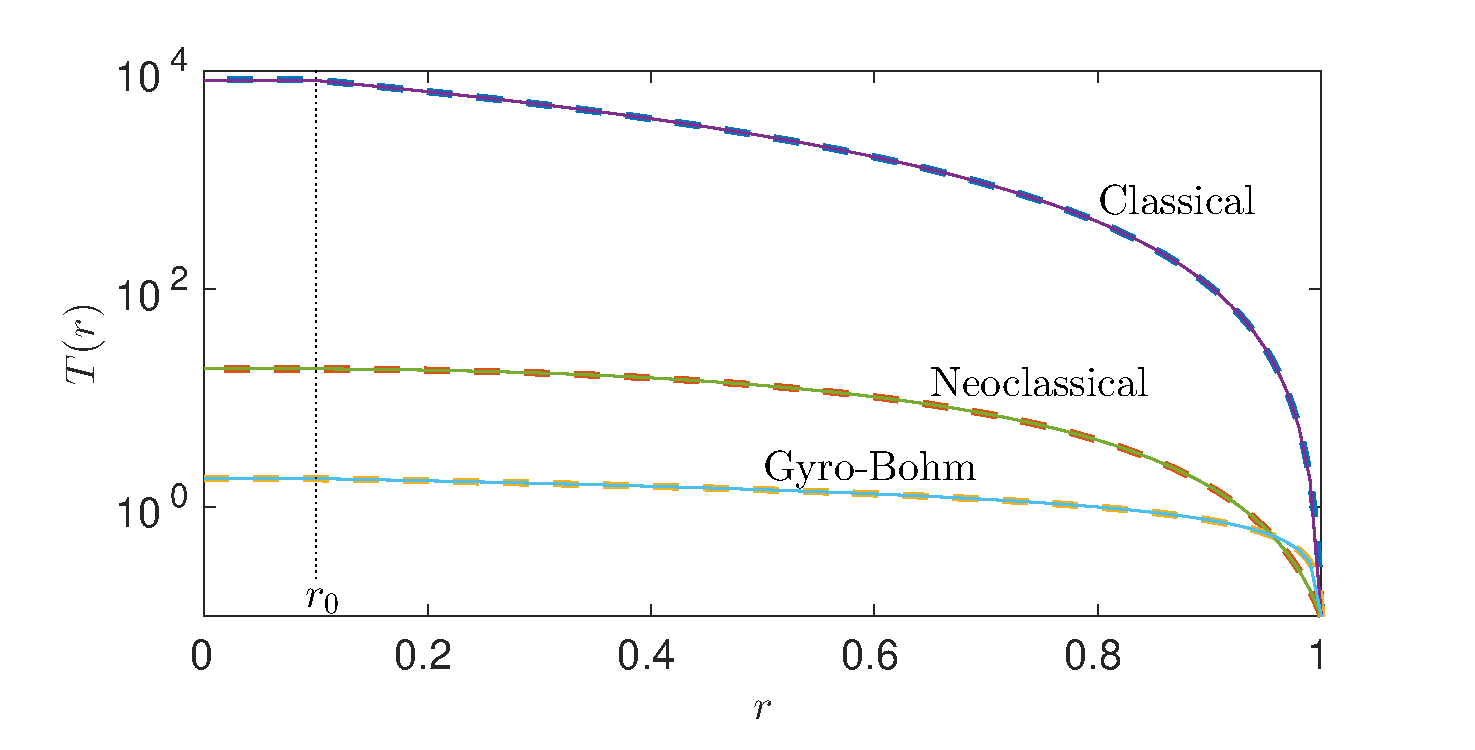
\includegraphics[width=12cm]{Q2.eps}
\caption{Temperature profiles for the three different types of heat
  transport, using the dimensionless values $S_0=10$, $R=1$,
  $r_0=0.1$, $T_0=0.1$, $\alpha_1=0.05$, $\alpha_2=0.5$ and
  $\alpha_3=5$. Also in the figure are numerical solutions to the
  differential equations shown as thick, dashed lines. Note the log
  scale on the vertical axis.}
\label{fig:transp}
\end{figure}

Using the dimensionless values $S_0=10$, $R=1$, $r_0=0.1$, $T_0=0.1$,
$\alpha_1=0.05$, $\alpha_2=0.5$ and $\alpha_3=5$. The core temperature
for the three different scenarios can be calculated to
\begin{equation}
\mathcal{T}\approx8\,160\qc
\mathscr{T}\approx18.5\qc
\mathfrak{T}\approx1.83,
\end{equation}
for classical, neoclassical and Gyro-Bohm transport
respectively. We clearly see that classical transport would have
yielded the, by almost three orders of magnitude, highest core
temperature, and that Gyro-Bohm yields the lowest core
temperature. This can also be seen in \figref{fig:transp}, where the
different temperature profiles have been plotted. 


\section{MHD stability}
Starting from the ideal MHD equations
\vspace{-22pt}
\begin{multicols}{2}
\begin{subequations}
\begin{align}
\label{eq:MHD-a}
&\rhom\dv{\vb*U}{t}=\vb*J\cross\vb*B-\grad P
\\ \label{eq:MHD-b}
&\pdv{\rhom}{t} +\div(\rhom\vb*U)=0
\\ \label{eq:MHD-c}
&\vb*E+\vb*U\cross\vb*B=0
\end{align}
\end{subequations}

\columnbreak

\addtocounter{equation}{-1}
\begin{subequations}
\addtocounter{equation}{3}
\begin{align}
\label{eq:MHD-d}
&\dv{t}\qty[\frac{P}{\rhom}]=0
\\ \label{eq:MHD-e}
&\curl\vb*B=\mu_0\vb*J %\qc \div\vb*B=0
\\ \label{eq:MHD-f}
&\curl\vb*E=-\pdv{\vb*B}{t}
\end{align}
\end{subequations}
\end{multicols}\noindent
and linearizing all variables around a flow-less, static equilibrium:
\begin{equation}
\vb*U=\vb0+\epsilon\vb*U_1 \qc
\vb*J=\vb*J_0+\epsilon\vb*J_1 \qc
\vb*B=\vb*B_0+\epsilon\vb*B_1 \qc
\ldots
\end{equation}
we want to find the MHD stability equation
\begin{equation}
\rhom_0\pdv[2]{\vb*U_1}{t}=\vb*F(\vb*U_1).
\end{equation}

It seems clear that we should start with \eqref{eq:MHD-a} and
linearize it. To order $\epsilon$ we get
\begin{equation}\label{eq:MHD-a-lin}
\rhom_0\dv{\vb*U_1}{t} = 
\vb*J_1\cross\vb*B_0+\vb*J_0\cross\vb*B_1-\grad P_1.
\end{equation}
Note that the term $\rhom_1\dv*{\vb*U_0}{t}=\vb0$, since
$\vb*U_0\equiv\vb0$. We further note that a full time derivative can
be written as
\begin{equation}
\dv{f}{t}=\pdv{f}{t}+\vb*U\vdot\grad{f},
\end{equation}
and when linearized
\begin{equation}\label{eq:dv-lin}
\dv{f_0}{t}+\epsilon\dv{f_1}{t}=
\pdv{f_0}{t}
+\epsilon\qty[\pdv{f_1}{t}+\vb*U_1\vdot\grad{f_0}]
+\order{\epsilon^2}.
\end{equation}
Once again $\vb*U_0\equiv\vb0$ was used.
In \eqref{eq:MHD-a-lin}, the full derivative therefore becomes
\begin{equation}\label{eq:dvU1}
\dv{\vb*U_1}{t}=\pdv{\vb*U_1}{t}+\vb*U_1\vdot\grad\vb*U_0
=\pdv{\vb*U_1}{t}.
\end{equation}
If we therefore operate with a \emph{partial} time derivative on
\eqref{eq:MHD-a-lin}, with \eqref{eq:dvU1} in mind, we get
\begin{equation}\label{eq:MHD-stab1}
\rhom_0\pdv[2]{\vb*U_1}{t} = 
\pdv{\vb*J_1}{t}\cross\vb*B_0
+\vb*J_0\cross\pdv{\vb*B_1}{t}-\grad \pdv{P_1}{t}.
\end{equation}
Here we have used the fact that the unperturbed state is static,
meaning that $X_0$ is constant in time for any variable $X$. We have
also used the fact that different (partial) derivatives commute, i.e. 
$\pdv*{(\grad P_1)}{t}=\grad\pdv*{P_1}{t}$.

From here we can use \eqref{eq:MHD-e}, \eqref{eq:MHD-f} and
\eqref{eq:MHD-c} to get 
\begin{equation}
\pdv{\vb*J_1}{t}=\frac{1}{\mu_0}\curl\pdv{\vb*B_1}{t}
=\frac{1}{\mu_0}\curl\qty[-\curl\vb*E_1]
=-\frac{1}{\mu_0}\curl\qty[\curl\qty(-\vb*U_1\cross\vb*B_0)].
\end{equation}
When linearizing \eqref{eq:MHD-c}, $\vb*U_0\equiv\vb0$ was used. 
Next up we can use \eqref{eq:MHD-f} and \eqref{eq:MHD-c} to get
\begin{equation}
\pdv{\vb*B_1}{t}=-\curl\vb*E_1
=-\curl\qty(-\vb*U_1\cross\vb*B_0).
\end{equation}
This, together with $\mu_0\vb*J_0=\curl\vb*B_0$, inserted into
\eqref{eq:MHD-stab1} yields
\begin{equation}\label{eq:MHD-stab2}
\begin{aligned}
\rhom_0\pdv[2]{\vb*U_1}{t} =& 
\frac{1}{\mu_0}\qty{\curl\qty[\curl\qty(\vb*U_1\cross\vb*B_0)]}
\cross\vb*B_0+\\
&+\frac{1}{\mu_0}(\curl\vb*B_0)\cross
\qty[\curl\qty(\vb*U_1\cross\vb*B_0)]
&-\grad \pdv{P_1}{t}.
\end{aligned}
\end{equation}

Now we turn our attention to the last term. We have a (partial) time
derivative of $P_1$, which suggests that we should use
\eqref{eq:MHD-d}. Note the full derivative meaning that we have to
use \eqref{eq:dv-lin},
%This results in
%\begin{equation}
%\dv{f_1}{t}=\pdv{f_1}{t}+\vb*U_1\vdot\grad{f_0},
%\end{equation}
where
\begin{equation}
f=\frac{P_0+\epsilon P_1}{(\rhom_0+\epsilon\rhom_1)^\gamma}
=\frac{P_0}{\rhom_0^\gamma}+\epsilon\qty[
\frac{P_1}{\rhom_0^\gamma} 
-\gamma\frac{P_0}{\rhom_0^\gamma}\frac{\rhom_1}{\rhom_0}].
\end{equation}
It is therefore clear that
\begin{equation}
f_0=\frac{P_0}{\rhom_0^\gamma}
\qc\qquad
f_1=\frac{P_1}{\rhom_0^\gamma} 
-\gamma\frac{P_0}{\rhom_0^{(\gamma+1)}}\rhom_1
\end{equation}
We can now see that the linearized \eqref{eq:MHD-d} becomes
\begin{equation}
\begin{aligned}
0=&\dv{f_1}{t}=\pdv{f_1}{t}+\vb*U_1\vdot\grad{f_0}\\
=&\frac{1}{\rhom_0^\gamma}\pdv{P_1}{t}
-\gamma\frac{P_0}{\rhom_0^{(\gamma+1)}}\pdv{\rhom_1}{t}
+\vb*U_1\vdot\qty[\frac{1}{\rhom_0^{\gamma}}\grad(P_0)
-\gamma\frac{P_0}{\rhom_0^{(\gamma+1)}}\grad(\rhom_0)],
\end{aligned}
\end{equation}
which can be rewritten as
\begin{equation}
\pdv{P_1}{t}=\gamma\frac{P_0}{\rhom_0}
\qty(\pdv{\rhom_1}{t}+\vb*U_1\vdot\grad\rhom_0)
-\vb*U_1\vdot\grad P_0.
\end{equation}
We now use \eqref{eq:MHD-b} and get
\begin{equation}
\pdv{\rhom_1}{t}=-\div(\rhom_0\vb*U_1)
=-\grad(\rhom_0)\vdot\vb*U_1
-\rhom_0\div\vb*U_1,
\end{equation}
which means that
\begin{equation}
\pdv{P_1}{t}=-\gamma P_0\div\vb*U_1
-\vb*U_1\vdot\grad P_0.
\end{equation}

We can now write \eqref{eq:MHD-stab2} as
\begin{equation}\label{eq:MHD-wave}
\begin{aligned}
\rhom_0\pdv[2]{\vb*U_1}{t} =& 
\frac{1}{\mu_0}\qty{\curl\qty[\curl\qty(\vb*U_1\cross\vb*B_0)]}
\cross\vb*B_0+\\
&+\frac{1}{\mu_0}(\curl\vb*B_0)\cross
\qty[\curl\qty(\vb*U_1\cross\vb*B_0)]
+\grad\qty[\gamma P_0\div\vb*U_1+\vb*U_1\vdot\grad P_0],
\end{aligned}
\end{equation}
which is the full MHD stability/wave equation. 


\section{Alfvén waves in infinite, homogeneous plasmas}
Now we want to find harmonic solutions,
$\vb*U_1\propto\vb*V_1(\vb*r)\ee^{\pm\ii\omega t}$, to
\eqref{eq:MHD-wave} in a uniform and static plasma. The static
assumption has already been heavily used in the previous problem to
derive \eqref{eq:MHD-wave}. The uniform assumption however, will help
us with the fact that $X_0$ is constant is space as well, for any
variable $X$; especially $\curl\vb*B_0=0$ and $\grad P_0=0$. With
these observations, \eqref{eq:MHD-wave} can be written as
\begin{equation}
-\rhom_0\omega^2\vb*V_1(\vb*r)
=\frac{1}{\mu_0}
\qty{\curl\qty[\curl\qty(\vb*V_1\cross\vb*B_0)]}\cross\vb*B_0
+\gamma P_0 \grad(\div\vb*V_1).
\end{equation}
This can be further simplified using the identity
\begin{equation}\label{eq:curl-cross}
\curl(\vb*F\cross\vb*G)
=(\vb*G\vdot\grad)\vb*F - (\vb*F\vdot\grad)\vb*G
+\vb*F(\div\vb*G) - \vb*G(\div\vb*F),
\end{equation}
which gives
$\curl(\vb*V_1\cross\vb*B_0)
=(\vb*B_0\vdot\grad)\vb*V_1 - \vb*B_0(\div\vb*V_1)$
since $\vb*B_0$ is constant.Thus
\begin{equation}
-\rhom_0\omega^2\vb*V_1(\vb*r)
=\frac{1}{\mu_0}
\qty{\curl\qty[(\vb*B_0\vdot\grad)\vb*V_1 
- \vb*B_0(\div\vb*V_1)]}\cross\vb*B_0
+\gamma P_0 \grad(\div\vb*V_1).
\end{equation}
Now we can also choose our coordinate system such that
$\vb*B_0=B_0\vu{z}$. This gives
\begin{equation}\label{eq4:MHD-wave_real}
-\omega^2\vb*V_1(\vb*r)
=\vA^2\qty{\curl\qty[\pdv{z}\vb*V_1 
- \vu{z}(\div\vb*V_1)]}\cross\vu{z}
+\cs^2 \grad(\div\vb*V_1),
\end{equation}
where
\begin{equation}
\vA^2:=\frac{B_0^2}{\mu_0\rhom_0}\qc\quad
\cs^2:=\frac{\gamma P_0}{\rhom_0}
\end{equation}
are the Alfvén velocity and the sound speed respectively.

Now, since the plasma is uniform and static, we can use the Fourier
transform
\begin{equation}
\vb*V_1(\vb*r)=\frac{1}{(2\pi)^3}
\int \rd^3k\, \vb*W(\vb*k)\,\ee^{+\ii\vb*k\vdot\vb*r},
\end{equation}
which means that $\grad\to\ii\vb*k$. We can furthermore rotate our
coordinate system such that $\vb*k=k_{||}\vu{z}+k_\perp\vu{y}$. We
can therefore write \eqref{eq4:MHD-wave_real} as
\begin{equation}
\begin{aligned}
-\omega^2\vb*W(\vb*k)
=&-\vA^2\qty{\vb*k\cross\qty[k_{||}\vb*W 
- (\vb*k\vdot\vb*W)\vu{z}]}\cross\vu{z}
-\cs^2 (\vb*k\vdot\vb*W)\vb*k\\
=&-\vA^2k_{||}[(\vb*k\cross\vb*W)\cross\vu{z}]
+\vA^2(\vb*k\vdot\vb*W)[(\vb*k\cross\vu{z})\cross\vu{z}]
-\cs^2 \vb*k(\vb*k\vdot\vb*W).
\end{aligned}
\end{equation}
Now we use the vector triple product identity
\begin{equation}
(\vb*a\cross\vb*b)\cross\vb*c=
(\vb*a\vdot\vb*c)\vb*b
-(\vb*b\vdot\vb*c)\vb*a,
\end{equation}
and move $\omega^2\vb*W$ to the RHS, which yields
\begin{equation}
\vb0=
\qty(\omega^2-\vA^2k_{||}^2)\vb*W+\vA^2k_{||}W_z\vb*k
-\qty[\qty(\vA^2+\cs^2)k_\perp\vu{y}+\cs^2k_{||}\vu{z}
](\vb*k\vdot\vb*W).
\end{equation}
This then simplifies down to
\begin{equation}\label{eq:MHD-unif-disp}
\begin{bmatrix}
\omega^2-\vA^2k_{||}^2 & 0 & 0 \\
0 & \omega^2-\vA^2k^2-\cs^2k_\perp^2 & -\cs^2k_{||}k_\perp\\
0 & -\cs^2k_{||}k_\perp & \omega^2 -\cs^2k_{||}^2
\end{bmatrix}
\begin{bmatrix}
W_x\\W_y\\W_z
\end{bmatrix}
=
\begin{bmatrix}
0\\0\\0
\end{bmatrix},
\end{equation}
where $k^2=|\vb*k|^2=k_{||}^2+k_\perp^2$. 

We get non-trivial solutions only when the determinant is 0, i.e.
\begin{equation}
\begin{aligned}
0=&\qty(\omega^2-\vA^2k_{||}^2)\qty[
\qty(\omega^2-\vA^2k^2-\cs^2k_\perp^2)\qty(\omega^2 -\cs^2k_{||}^2)
-\qty(-\cs^2k_{||}k_\perp)^2]\\
=&\qty(\omega^2-\vA^2k_{||}^2)\qty[\omega^4-
\qty(\vA^2k^2+\cs^2k_\perp^2+\cs^2k_{||}^2)\omega^2
+\vA^2k^2\cs^2k_{||}^2
+\cs^4k_\perp^2k_{||}^2-\qty(\cs^2k_{||}k_\perp)^2]\\
=&\qty(\omega^2-\vA^2k_{||}^2)\qty[
\omega^4-\qty(\vA^2+\cs^2)k^2\omega^2
+\vA^2\cs^2k^2k_{||}^2],
\end{aligned}
\end{equation}
which has the solutions
\begin{equation}\label{eq4:MHD-shear}
\omega^2=\vA^2k_{||}^2
\end{equation}
or
\begin{equation}
\begin{aligned}
\omega^2=&\frac{1}{2}\qty(\vA^2+\cs^2)k^2
\pm\sqrt{\frac{1}{4}\qty(\vA^2+\cs^2)^2k^4
-\vA^2\cs^2k^2k_{||}^2}\\
=&\frac{1}{2}\qty(\vA^2+\cs^2)k^2\qty[
1\pm\sqrt{1-\frac{4\vA^2\cs^2k_{||}^2}{\qty(\vA^2+\cs^2)^2k^2}}].
\end{aligned}
\end{equation}

We now see that \eqref{eq:MHD-unif-disp} has three different
modes. The first one being \eqref{eq4:MHD-shear}, which requires
$\vb*W=W\vu{x}$ and is therefore perpendicular to both $\vb*B_0$ and
$\vb*k$. Linearizing and Fourier transforming \eqref{eq:MHD-c} and
\eqref{eq:MHD-f} yields
\begin{equation}
\vb*B_1 = -\frac{\vb*k\cross(\vb*W\cross\vb*B_0)}{\omega}
=\frac{\cancel{(\vb*W\vdot\vb*k)}\vb*B_0
-(\vb*B_0\vdot\vb*k)\vb*W}{\omega}
=-\frac{(\vb*B_0\vdot\vb*k)}{\omega}\vb*W.
\end{equation}
In other words, $\vb*B_1$ is perpendicular to $\vb*B_0$. This wave
mode shifts the the magnetic field lines perpendicularly to their
original direction (shearing), which is why it is called the
\emph{shear Alfvén wave}. We can further more see that 
if $\vb*k\vdot\vb*W=0$ (which implies $\div\vb*V_1=0$) then the plasma
becomes \emph{incompressible}. By linearizing \eqref{eq:MHD-b}, we get  
\begin{equation}
0=\pdv{\rhom_1}{t} + \vb*V_1\vdot\grad\rhom_0
+\cancel{\rhom_0\,\div\vb*V_1}
=\dv{\rhom_1}{t}.
\end{equation}
That is the density is constant in time to first order, i.e. the
plasma does not compress -- loosely talking it's \emph{incompressible}
under this wave mode. 


\section{Alfvén waves in a sheared magnetic field}
\newcommand{\wA}{\omega_{\text{A}}}
Assuming that the plasma is incompressible, $\div\vb*U=0$, and that
the unperturbed magnetic field is given by
\begin{equation}\label{eq5:B0}
\vb*B_0(x)=B_{0y}(x)\vu{y}+B_{0z}(x)\vu{z},
\end{equation}
we want to show that the shear Alfvén wave mode dispersion relation is
\begin{equation}\label{eq5:want}
\dv{x}\qty[\qty(\omega^2-\wA^2(x))\dv{W_x}{x}]
-k^2\qty(\omega^2-\wA^2(x))W_x(x)=0,
\end{equation}
where $\vb*W$ is the sesqui-Fourier amplitude of the first order
perturbed velocity
\begin{equation}
\vb*U_1(x, y, z; t) = \vb*W(x)\ee^{\ii(k_yy+k_zz-\omega t)}.
\end{equation}

\subsection{Finding the dispersion relation}
Since apparently \eqref{eq5:B0} makes the MHD system over-determined,
we can scrap the adiabatic equation of state, and with it the
pressure.\footnotemark{} We can therefore write \eqref{eq:MHD-wave} as
\begin{equation}
\begin{aligned}
\rhom_0\pdv[2]{\vb*U_1}{t} =& 
\frac{1}{\mu_0}\qty{\curl\qty[\curl\qty(\vb*U_1\cross\vb*B_0)]}
\cross\vb*B_0+\\
&+\frac{1}{\mu_0}(\curl\vb*B_0)\cross
\qty[\curl\qty(\vb*U_1\cross\vb*B_0)].
\end{aligned}
\end{equation}
\footnotetext{I'm not fully convinced that \eqref{eq5:B0} is single
  handedly responsible for us being able to scrap the pressure, but I
  guess it also has something to do with the fact that we're only
  studying the shear mode.}

From here we have to start simplifying things. We can begin with the
simplest term first
\begin{equation}
\curl\vb*B_0=\pdv{x}\vu{x}\cross
\qty[B_{0y}(x)\vu{y}+B_{0z}(x)\vu{z}]
=B_{0y}'(x)\vu{z}-B_{0z}'(x)\vu{y},
\end{equation}
where prime denotes differentiation with respect to $x$.
Then $\curl\qty(\vb*U_1\cross\vb*B_0)$, with \eqref{eq:curl-cross} we
get 
\begin{equation}
\begin{aligned}
\curl\qty(\vb*U_1\cross\vb*B_0) 
=& (\vb*B_0\vdot\grad)\vb*U_1
- (\vb*U_1\vdot\grad)\vb*B_0\\
=&B_{0y}\pdv{\vb*U_1}{y}+B_{0z}\pdv{\vb*U_1}{z}
-U_{1x}\pdv{\vb*B_0}{x}\\
\to& (k_y B_{0y} + k_z B_{0z}) \vb*W 
-W_{x}\qty(B_{0y}'(x)\vu{y} + B_{0z}'(x)\vu{z}),
\end{aligned}
\end{equation}
where the two last terms in \eqref{eq:curl-cross} vanish since
$\div\vb*U=\div\vb*B=0$. Next, using the identity
\begin{equation}
\curl(f\vb*G) = (\grad f)\cross\vb*G+f\curl\vb*G,
\end{equation}
we can write
\begin{equation}
\curl\qty[\curl\qty(\vb*U_1\cross\vb*B_0)]
\to \Big(k_yB_{0y}+k_zB_{0z}\Big)(\curl\vb*W)
+\Big(k_yB_{0y}'+k_zB_{0z}'\Big)\vu{x}\cross\vb*W,
\end{equation}
where $\curl\vb*W=[(\pdv*{x})\vu{x}+k_y\vu{y}+k_z\vu{z}]\cross\vb*W$.

Now assuming\footnotemark{} that $\vb*W=W\vu{x}$, what I seem to end
up with (after a good deal of vector calculus) is
\footnotetext{This is probably wrong, but it's late Sunday night, and
  I've had enough och vector calculus...}
\begin{equation}
\begin{aligned}
-\rhom_0\omega^2W\vu{x}=
\frac{1}{\mu_0}\Bigg\{&\qty[(k_yB_{0y}+k_zB_{0z})^2
-(B_{0y}B_{0y}''+B_{0z}B_{0z}'')
+\qty({B_{0y}'}^2+{B_{0z}'}^2)]W\\
&+\qty[B_{0y}B_{0y}'+B_{0z}B_{0z}']W'
\Bigg\}\vu{x}\quad
 +\ldots\vu{y} +\ldots\vu{z}.
\end{aligned}
\end{equation}
With some extra crap on the $y$ and $z$ components on the RHS. The
lack of $W_x''$ terms also seems to suggest that $\vb*W=W\vu{x}$ is
not valid.

I had hoped that I would at least have gotten my hands on what $\wA$
would be, but not even that. There is however some dimensionally sound
alternatives here, however the only one which seem to have the right
sign seems to be 
\begin{equation}
\wA^2\stackrel{?}{=}\frac{{B_{0y}'}^2+{B_{0z}'}^2}{\mu_0\rhom_0}.
\end{equation}
It feels right and it is dimenionally sound, so that's my guess. 

\subsection{Singularity at $\omega=\wA$}
We can rewrite \eqref{eq5:want} as
\begin{equation}\label{eq5:ODE-B}
\qty(\omega^2-\wA^2(x))(W_x''-k^2W_x)-2\wA(x)\wA'(x)W_x'=0.
\end{equation}
Next, for $\omega\approx\wA$, we can take
\begin{equation}
\wA(x)=\omega+\xi\wA'(x_0)+\order{\xi^2},
\end{equation}
where $\xi=(x-x_0)\ll1$ and $x_0$ is such that $\wA(x_0)=\omega$. We can
write \eqref{eq5:ODE-B} as
\begin{equation}\label{eq5:ODE-B2}
-2\omega\wA'(x_0)\xi(W_x''-k^2W_x)-2\wA\wA'(x_0)W_x'=0.
\end{equation}
Now if\footnotemark{} $W_x(\xi)\sim\log(\xi)$ for $\xi\ll1$, then we
can write the RHS of \eqref{eq5:ODE-B2} as
\begin{equation}
\text{RHS[\eqref{eq5:ODE-B2}]}\sim
-2\omega\wA'(x_0)\xi\qty[\cancel{-\frac{1}{\xi^2}}-k^2\log(\xi)]
-\cancel{2\wA\wA'(x_0)\frac{1}{\xi}}
\sim2\omega\wA'(x_0)k^2\xi\log(\xi),
\end{equation}
and since $\xi\log(\xi)\to0$ as $\xi\to0$, we know that
$W_x\sim\log(\xi)$, that is $W_x$ asymptotically approaches
$\log(\xi)$ as $\xi\to0$ -- or in layman's terms $W_x$ is
logaritmically singular as when $\omega=\wA$.
\footnotetext{Note that we could have arrived at this conclusion
  without prior knowledge of the singularity. Since singularities
  become worse the more derivative that are applied, we would have
  known that the \emph{dominant balance} in \eqref{eq5:ODE-B2} would
  be between $\xi W_x''$ and $W_x'$, which gives $W_x\sim\log(\xi)$.
  \label{fnt:sing}}

\subsection{Higher order derivatives}
To mitigate the singularity when $\omega=\wA$, we need to consider
non-ideal MHD, which effectively introduces a fourth order derivative,
\begin{equation}
\eta W_x^{(4)}-2\omega\wA'(x_0)\xi(W_x''-k^2W_x)-2\wA\wA'(x_0)W_x'=0,
\end{equation}
where $\eta$ is small. By the same reasoning as in
footnote~\ref{fnt:sing} (even though we don't have a singularity) we
would assume a dominant balance between $\eta W_x^{(4)}$ and
$2\wA\wA'(x_0)W_x'$, from there we would be able to build up an
asymptotic series. If that doesn't work, then another technique from
asymptotic analysis is to express
\begin{equation}
W_x(\xi)=\ee^{S(\xi)}
\end{equation}
and then finding an asymptotic expansion for $S$ near $\xi=0$.

%%%%%%%%%%%%%%%%%%%%%%%%%%%%%%%%%%%%%%%%%%%%%%%%%%%%%%%%%%%%%%%%%%%%%%
\end{document}%% ^ ^ ^ ^ ^ ^ ^ ^ ^ ^ ^ ^ ^ ^ ^ ^ ^ ^ ^ ^ ^ ^ ^ ^ ^ ^ ^
%%%%%%%%%%%%%%%%%%%%%%%%%%%%%%%%%%%%%%%%%%%%%%%%%%%%%%%%%%%%%%%%%%%%%%
%  LocalWords: Alfvén MHD Bohm quadratically incompressible
%  LocalWords:  logaritmically
